\section{Introduction}

We humans exhibit a remarkable ability to learn new concepts fast and efficiently. This ability is in stark contrast with conventional supervised machine learning, which is data hungry and requires a plethora of data points to develop an effective model. Meta-learning reframes the traditional machine learning problem, allowing machine learning models to learn utilising only a few examples. Humans have an innate capability to \textit{learn how to learn}, and bridging this gap between human and machine learning is beneficial, particularly in domains where data availability or acquisition is difficult, such as the drug-discovery domain. The main goal in the drug-discovery process is the identification and development of active compounds, that exhibit therapeutic effects against biological targets. The drug-discovery process comes with exorbitant costs and resource expenditure, which can exceed one billion dollars and take up to 15 years to complete \cite{hughes2011principles}. Moreover, data is also expensive and difficult to acquire, as this requires testing of numerous compounds both \textit{in-vitro} and (later) \textit{in-vivo}. Even upon identification of leads, attrition rates are high as the compound usually fails for other reasons such as poor absorption, distribution, metabolism, excretion, or toxicology (ADMET) characteristics \cite{waring2015analysis}. It is difficult to predict such characteristics about the candidate molecule when only a small amount of related biological data is available. Therefore, the lead identification and optimisation step in drug discovery is essentially a low-data problem \cite{altae2017low}, in contrast to conventional machine learning which is data-hungry. In recent years, the computer vision domain saw successful applications and advancements for low-data machine learning \cite{koch2015siamese, vinyals2016matching, snell2017prototypical, sung2018learning}. Few-shot learning relieves the burden of collecting large-scale labelled data and makes the learning of rare cases possible \cite{wang2020generalizing}. 

\begin{figure}
	\centering
	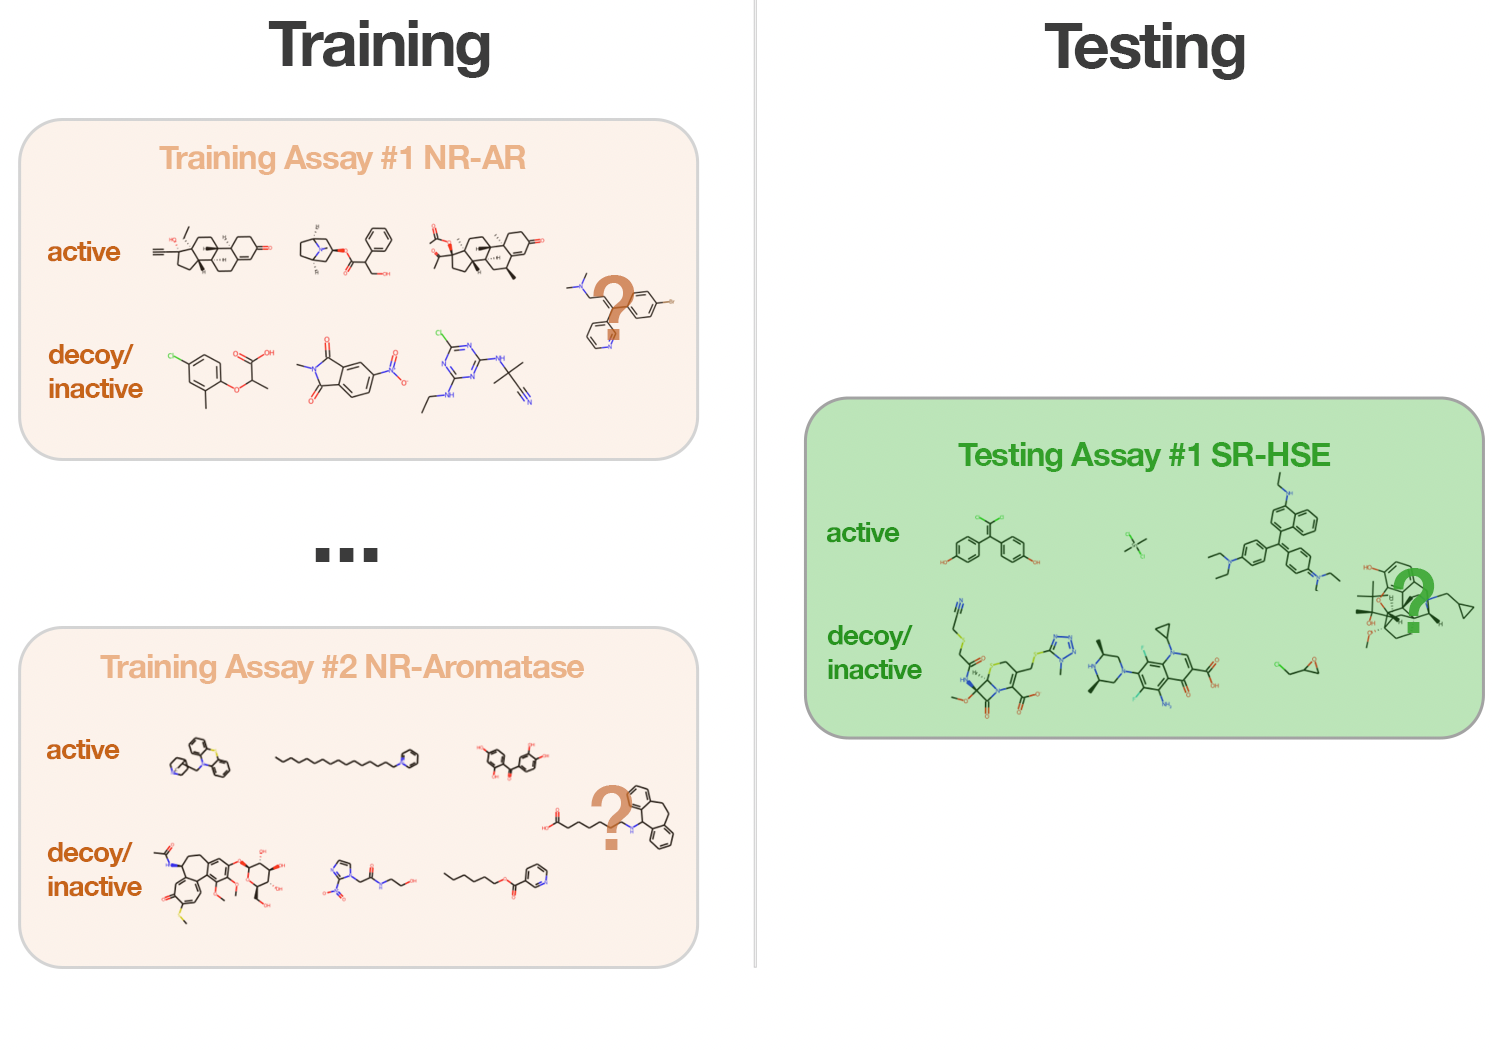
\includegraphics[width=0.8\linewidth]{img/tox21-metalearning.png}
	\caption{2-way 3-shot few-shot classification. Training a meta-learner on a set of experimental assays, and generalising for an unseen assay in the Tox-21 dataset.}
	\label{fig:tox21metalearning}
\end{figure}

Building on this notion, we aim to explore few-shot learning to address the low-data problem for hit identification and lead optimisation. The ability for a machine learning model to learn new concepts fast with just a few training examples is invaluable for this domain, where data on active compounds is scarce. Meta-learning aims to achieve generalising capabilities for environments that were previously unseen during training time. Few-shot classification, a meta-learning paradigm, we train models using a variety of training tasks and optimise for classification performance over a distribution of tasks, including unseen ones. Learning consists of a series of episodes, each consisting of an \textit{N}-way \textit{K}-shot classification task, effectively simulating the conditions at testing time. The \textit{way} refers to the number of classes we have per task and the \textit{shot} component refers to the number of samples. These samples make up the support set \cite{snell2017prototypical}. During test time, a small support set is sampled from new, previously unseen targets, and these few data points are used by the model to generalise for the activity of query molecules against this new target \cite{vinyals2016matching}. Figure~\ref{fig:tox21metalearning} shows an example of a typical meta-learning scenario on the Tox21 dataset \citep{huang2016tox21challenge}, where data from a set of assays reserved for training are used to train a model, which is later used to generalise for a new, unseen assay using only a support set from this new assay. We highlight that few-shot learning in the hit identification and lead optimisation is different to other domains such as computer vision, where the trained model recognises new classes. For example, given a few images of a lion as the support set, a class unseen during training, the model must generalise for new images of a lion. In the domain under study, the challenge is to train a model that is able to generalise for the behaviour of molecules in experimental assays which are related but not identical to the assays in the training collection, using only a small support set from this new experimental assay. The molecules used during testing can thus be previously seen during training, but only in the context of their activity for different, but related experimental assays. Given a few molecules from new experimental assays, can the model predict the activity of molecules in this new assay using molecular data for different, but related, targets as training data?

Molecules are complex structures, consisting of atoms and bonds, and which must be somehow represented in computational space. The classical notation of compounds is the empirical formula such as $C_3H_7NO_2$, however, this holds no specific information on the molecule's topology. In fact, this particular formula can refer to alanine, sarcosine, and lactamide. Molecular representations such as Extended-Connectivity Fingerprints (ECFP) \cite{rogers2010extended} and graph convolution learned embeddings \cite{duvenaud2015convolutional} embed more information than the empirical formula on the properties of the molecule, and can be used as inputs to machine learning networks. In this study, we mainly explore the use of graphs as embeddings for the low-data machine learning networks. A graph is formally defined as a set of nodes and a set of edges, where each edge connects a pair of nodes. This notion intuitively translates to molecular representations where atoms form the set of nodes, and the bonds form the set of edges. Graphs are 2D objects, so spatial properties of a molecule such as bond angles and chirality are not inherent to the data object, but are instead encoded as node or edge attributes \cite{david2020molecular}. Embeddings of molecular graphs, augmented with atom feature information, can be learned using graph convolutional neural networks, which could be of benefit over topological molecular representations such as ECFP \cite{wu2018moleculenet}. 

In this study, we explore the application of several few-shot learning architectures including, in chronological order, Siamese Networks \citep{koch2015siamese}, Matching Networks \citep{vinyals2016matching}, Prototypical Networks \citep{snell2017prototypical}, and Relation Networks \citep{sung2018learning}. This group of architectures fall under the umbrella of metric-based meta-learning. In our study, we embed molecule representations using graph convolution networks, and then use or learn a distance function over these embeddings. Effectively, metric-based learners seek to learn a relationship between the input embeddings in the task space. For the purposes of this study, few-shot learning refers to training with as little as one example per class, referred to as one-shot learning \cite{koch2015siamese, vinyals2016matching}, to a maximum of ten examples per class. 

\section{Related Work}

Several successful research undertakings have exploited the low-data learning paradigm, especially in the computer-vision domain \cite{koch2015siamese, vinyals2016matching, snell2017prototypical, sung2018learning}. Being able to learn from only a few examples is especially important in domains that suffer from a paucity of data. This inaccessibility could be attributed to privacy, safety, or ethical issues, in addition to other issues such as the time, resources and exorbitant costs associated with data acquisition. Learning with low-data can lead to less expensive data gathering and reduced computational cost for learning \cite{wang2020generalizing}.

Building on past work in the metric-based meta-learning sphere \cite{vinyals2016matching}, \citet{altae2017low} introduce a deep-learning architecture for few-shot learning in drug discovery, in which they propose the iterative refinement long short-term memory (IterRefLSTM). IterRefLSTM builds on the Matching Networks \cite{vinyals2016matching} by introducing the Iterative Refinement of embeddings using Long-Short Term Memory (LSTM) networks. In our research, we build on the work by \citep{altae2017low} and extend it through the application of other successful few-shot learning approaches, previously explored for other domains such as the computer-vision domain. The authors employ Graph Neural Networks (GNN) to learn molecular embeddings, which are then fed into the low-data architectures for classification.

\subsection{Graph Neural Networks}

Molecules must be represented in computational space before processing them using few-shot machine learning techniques. \citet{wu2018moleculenet} report that graph-based models outperform conventional machine learning models on the majority of datasets, suggesting that a learned embedding is advantageous over other molecular representations. Thus, we opt for graph learned molecular representations to embed the input molecules. Graphs are natural representations of molecules, where nodes and edges represent atoms and bonds, respectively. When representing molecules, the set of vertices \textit{V} intuitively refers to atoms within a molecule, while the set of edges \textit{E} refers to the bonds that connects two atoms together (see Equation~\ref{eq_graph}). Selected properties such as atomic number, atom type, charge, and valences, amongst others, can be encoded in the node feature vector, in addition to bond information. However, the latter is omitted for the purpose of this study.

\begin{equation}\label{eq_graph}
	\mathcal{G}=(\mathcal{V}, \mathcal{E})
\end{equation}

Graph neural networks may be used to learn molecular representations \cite{jiang2021could}. Embeddings learned through neural networks afford the construction of automated features, rather than fixed fingerprints. Graph neural networks transform small molecules into real-valued vector representations, which are an effective way of processing small molecules via deep neural networks \cite{gomez2018automatic}. \citet{duvenaud2015convolutional} report that using a differentiable method reduces collisions of substructures, and the learned embedding can be optimised to contain relevant features such as biological activity and substructure information.

If the graph object is our input signal, we can apply a set of operators to approximate the function we are attempting to learn. \citet{bronstein2021geometric} propose four key building blocks for deep learning on graphs, which include linear set equivariant layers, non-linear functions, local pooling layers and set invariant layers. For graphs, the nodes $v$ are found on a domain $\Omega$ such that $v \in \Omega$. The nodes in $\Omega$ are stored in a feature space $C$, such that $C = \mathbb{R}^k$. Using a set of feature functions $X(\Omega, C)$, we can transform the feature space of the nodes in our domain. 

In the equivariant layer $B$, we can take the nodes in our domain and apply a function that transforms the features of the nodes such that $X(\Omega, C) \rightarrow X(\Omega', C')$. Equivariance allows for a function $g$ to be applied before or after this layer, such that $B(g.x) = g.B(x)$. The non-linear activation functions can be applied element-wise on the features of the nodes in a graph, such that $(\sigma(x))(v) = \sigma(x(v))$. Local pooling layers can be used to apply coarsening to the graph such that $X(\Omega, C) \rightarrow X(\Omega', C)$, in which we can reduce the number of nodes in our domain such that $\Omega' \subseteq \Omega$. Finally, we have the invariant layer $Z$, which can also be referred to as a global pooling layer, in which $X(\Omega, C) \rightarrow y$, which satisfies the invariant condition such that $Z(g.x) = Z(x)$ \citep{bronstein2021geometric}. Figure \ref{fig:neuralgraphfingerprint} illustrates an example of a GNN to learn a molecular embedding.

\begin{figure}[h]
	\centering
	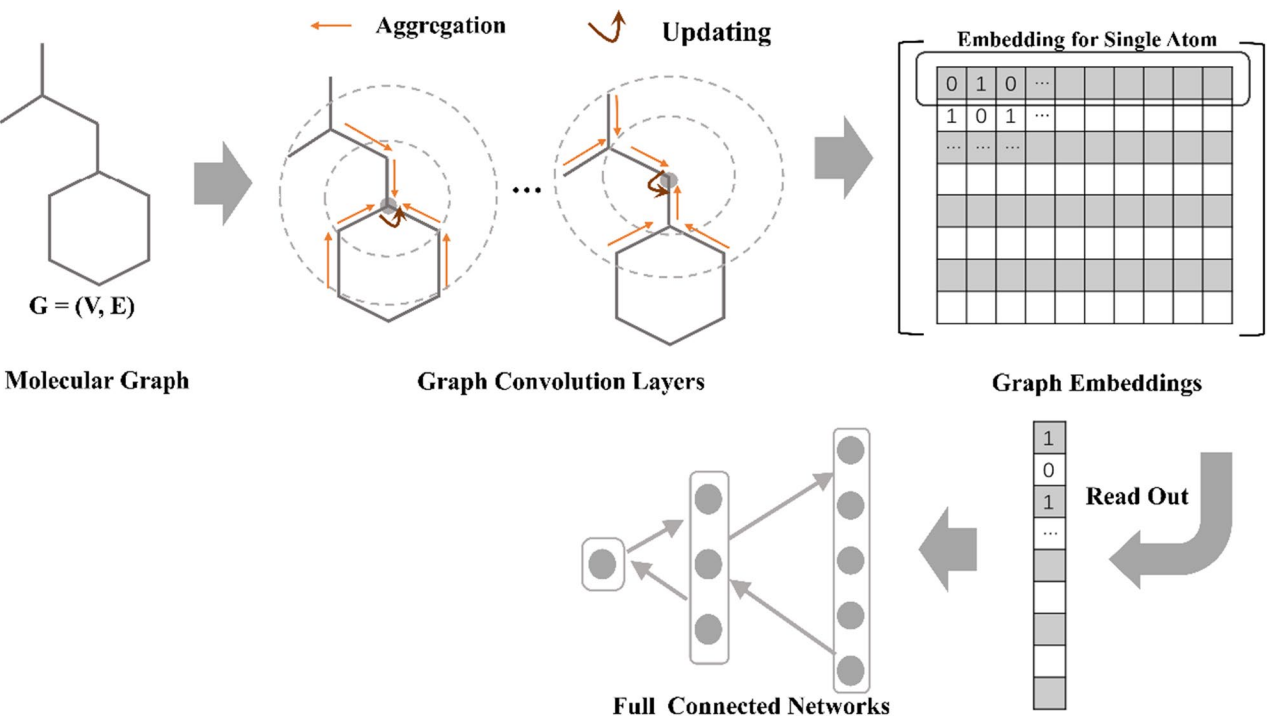
\includegraphics[width=0.9\linewidth]{img/graph_mol_embedding.png}
	\caption[Learned Embedding through a GCN]{A typical pipeline for representing molecules using a learned embedding function, which can be processed further using feed-forward neural networks as shown. Reproduced from \citet{jiang2021could}.}
	\label{fig:neuralgraphfingerprint}
  \end{figure}

\subsection{Metric-based Few-Shot Learning}

The success of a few-shot learning model for metric-based meta-learning is dependent on the effectiveness of a kernel $k_\theta$, which measures the similarity between data samples ${x..x_i}$ from a support set $S$ (see Equation \ref{kernel}) using a metric or distance function. The techniques employed in this study, excluding the benchmark model, use the support and query embeddings generated from the graph neural network to learn the kernel function.

\begin{equation}
	\label{kernel}
	P_\theta(y \vert \mathbf{x}, S) = \sum_{(\mathbf{x}_i, y_i) \in S} k_\theta(\mathbf{x}, \mathbf{x}_i)y_i
\end{equation}

\subsubsection{Siamese Networks}

Siamese networks \cite{bromley1993signature, koch2015siamese} are composed of two identical networks, with shared weights and parameters, taking in a pair of data samples as inputs. As the neural networks share weights, the feature extraction is maintained to the same feature space for both inputs. These identical subnetworks are finally connected in a final layer that acts as a distance function for the two outputs.

\begin{figure}[h]
	\centering
	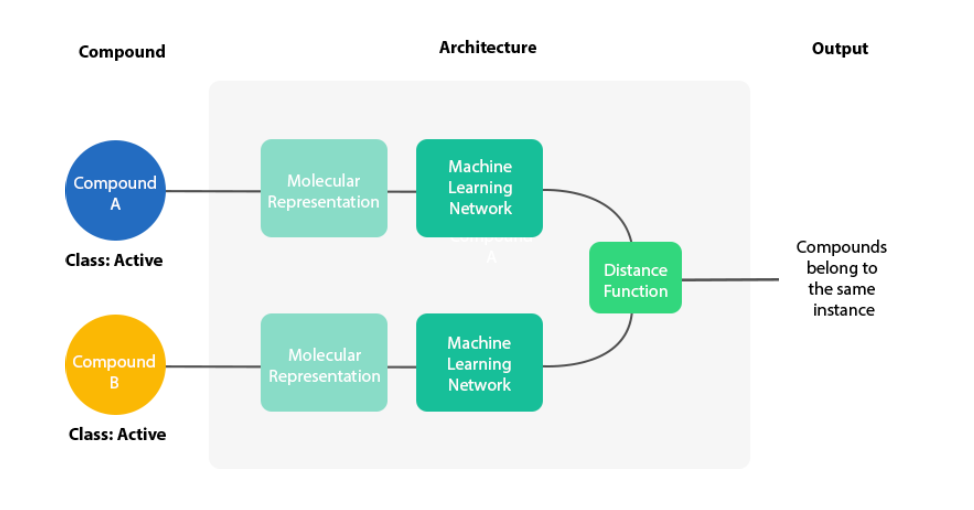
\includegraphics[width=0.9\linewidth]{img/high-level siamese.png}
	\caption[High-level schematic of Siamese network]{High level schematic of a Siamese network for molecular network. \index{High Level Schematic of Siamese Network}}
	\label{fig:siamesenetarchi}
\end{figure}

\subsubsection{Matching Networks}

Matching Networks \cite{vinyals2016matching} build on Siamese Networks, but instead of learning a metric function over pairs of data, the classifier learns how to define a probability distribution of output labels from query/test examples using a support set $S$. The classifier outputs a sum of attention weighted labels from the support set to predict the similarity between the test example and the samples from the support set. We use the same embedding function for the support and query sets to compute the molecular embeddings. Subsequently, the cosine similarity between pairs of data points between the support and query sets is computed, which is then normalised by a softmax function. The attention mechanism $a$ in $\hat{y} = \sum_{i=1}^{n} a(\hat{x}, x_i)y_i$ specifies how similar $\hat{x}$ is to each example $x$ in $S$.

\begin{figure}[!ht]
	\centering
	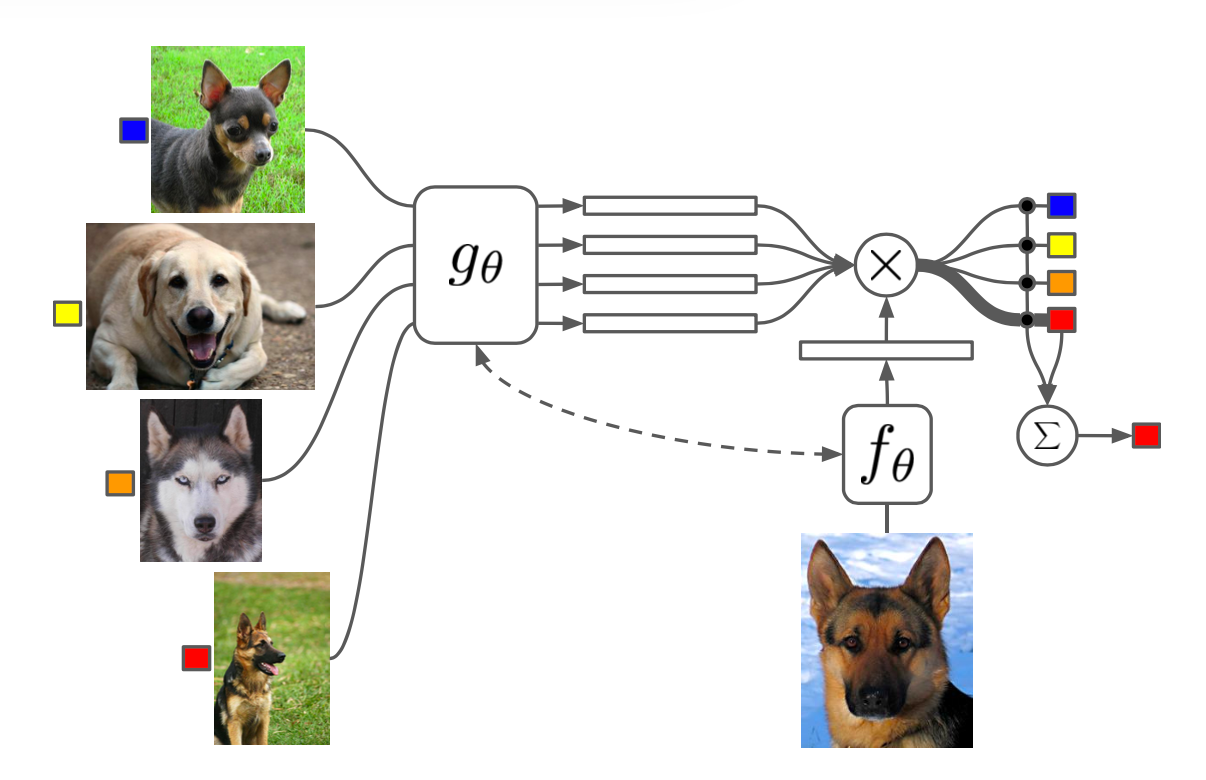
\includegraphics[width=0.7\linewidth]{img/matching_networks.png}
	\caption[Matching Networks Architecture]{Matching Networks Architecture. Reproduced from \citet{vinyals2016matching}.}
	\label{fig:matchingnets}
\end{figure}

Figure~\ref{fig:matchingnets} illustrates the Matching Nets architecture. Embedding functions $f$ and $g$ are Convolutional Neural Networks (CNNs) \citep{lecun1995convolutional}, potentially being identical to each other, which project the inputs to the feature space. \citet{vinyals2016matching} also propose full context embedding functions, which take as input the whole support set with the element $x_i$, thus resulting in \( g(x_i, S) \). Full context embeddings effectively modify how the element is embedded with respect to the whole support set $S$. A bidirectional LSTM is used to encode $x_i$ in the context of the support set. The attention mechanism $a$, at the end of the pipeline, is the classifier which takes a softmax over the cosine distance of the embeddings. 


\subsubsection{Prototypical Networks}

Prototypical Networks, proposed by \citet{snell2017prototypical}, are similar to Matching Networks. Instead of comparing the query support to each support data point, a \textit{prototype} is calculated, which takes all the support data points per class and creates an embedding by averaging over the embeddings related to each class, thus creating the \textit{prototypes}. The Euclidean distance between the query data point and the prototypes is calculated to classify the query (see Figure~\ref{fig:protonets}). In a one-shot learning scenario, Prototypical Networks are equivalent to Matching Networks, however, the Euclidean distance is used instead of the Cosine distance used in Matching Networks.

\begin{figure}[!ht]
	\centering
	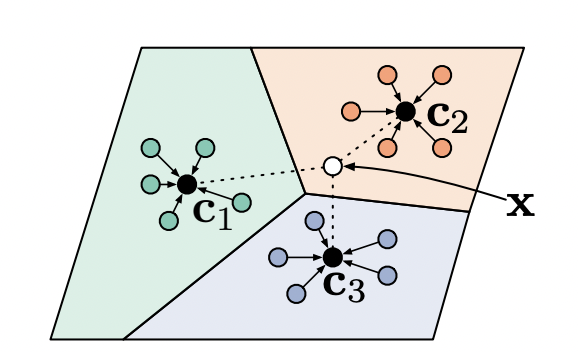
\includegraphics[width=0.7\linewidth]{img/protonets.png}
	\caption{Few-shot learning in Prototypical Networks, where prototypes \textbf{$c_k$} are taken as the mean of embedded support examples for each class. Reproduced from \citet{snell2017prototypical}.}
	\label{fig:protonets}
\end{figure}

\subsubsection{Relation Networks}

\citet{sung2018learning} present the Relation Network, a framework for few-shot learning, which could also be extended to zero-shot learning. The Relation Network learns a non-linear distance metric to compare support and query examples. As opposed to the aforementioned networks, this network uses a feed-forward neural network to learn a distance function in feature space. After embedding the support and query examples through an embedding function, each query example is concatenated with each of the feature maps. The resulting feature map concatenations are processed using a convolutional neural network to output a relation score vector, from which the class can be inferred (see Figure~\ref{fig:relationnets}).

\begin{figure}[h]
	\centering
	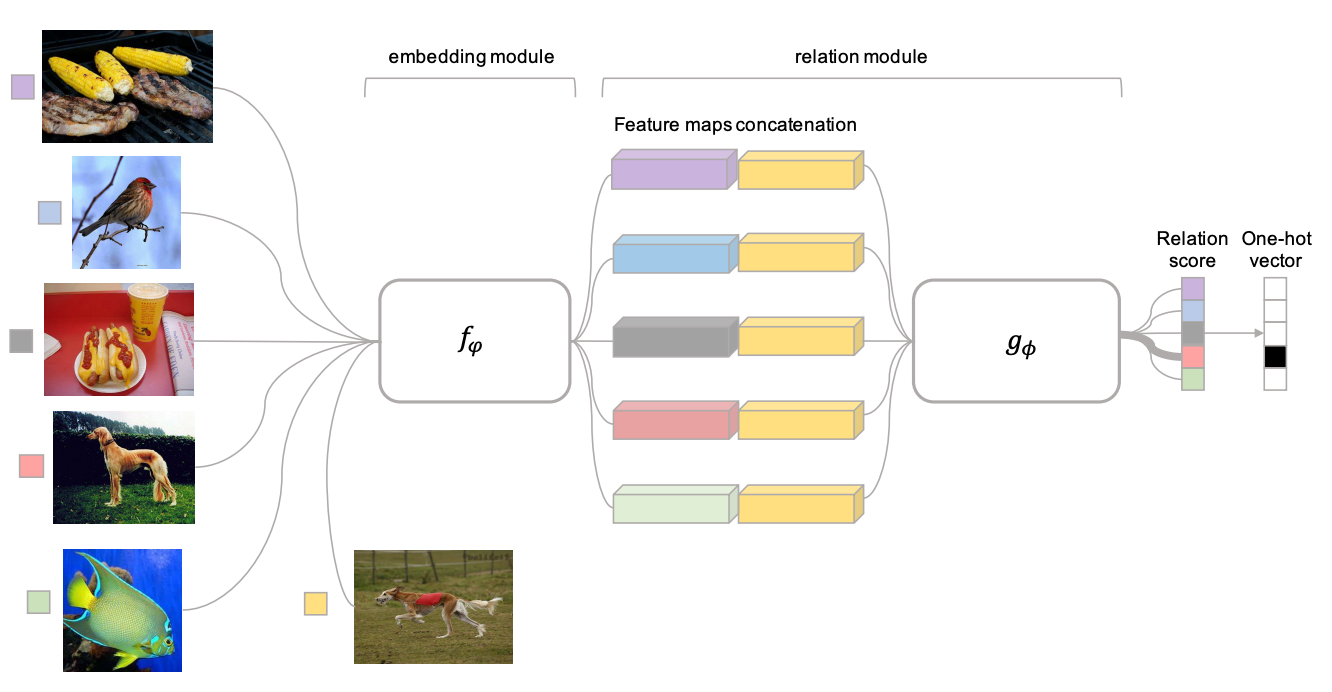
\includegraphics[width=0.9\linewidth]{img/relation-nets.png}
	\caption[Relation Networks]{Few-shot learning scenario in Relation Networks for a 5-way 1-shot learning task with one query as an example. Reproduced from \citet{sung2018learning}.}
	\label{fig:relationnets}
\end{figure}

\subsection{Iterative Refinement LSTM}

\citet{altae2017low} build on meta-learning concepts, where they train machine learning models on molecular data from a set of experimental assay targets (from the Tox21, SIDER, and MUV datasets) reserved for training. The model is then used to generalise for the activity of molecules in new, previously unseen experimental assays using only a small support set from the new assay. These test assays are related, but not identical, to the ones reserved for training. The number of molecules sampled for each class in the support set ranges from one to a maximum of ten molecules. In their work, the support and query molecules are embedded using a graph convolutional network.  Bond information and distinction between bond types was not considered in their study. We note that the \textit{pool} layers do not coarsen the graphs, but simply apply a max function over neighbouring nodes.

\citet{altae2017low} propose the iterative refinement long-short term memory (IterRefLSTM) to further process the resulting embeddings in a few-shot machine learning pipeline. In IterRefLSTMs two embedding functions $f(\dot|S)$ and $g(\dot|S)$ are developed simultaneously. Therefore, the embedding of the query is built iteratively with that of the support set, using information from the two sets to enhance both the support and query embeddings. Once the embeddings have been iteratively refined, the authors apply a metric-based function to classify the queries using the support set embeddings. To emulate the Matching Networks, the authors make use of the Cosine distance to compare embeddings. Figure \ref{fig:schematiconeshotdrug} illustrates a one-shot learning scenario encapsulating the aforementioned concepts.

\begin{figure}[h]
	\centering
	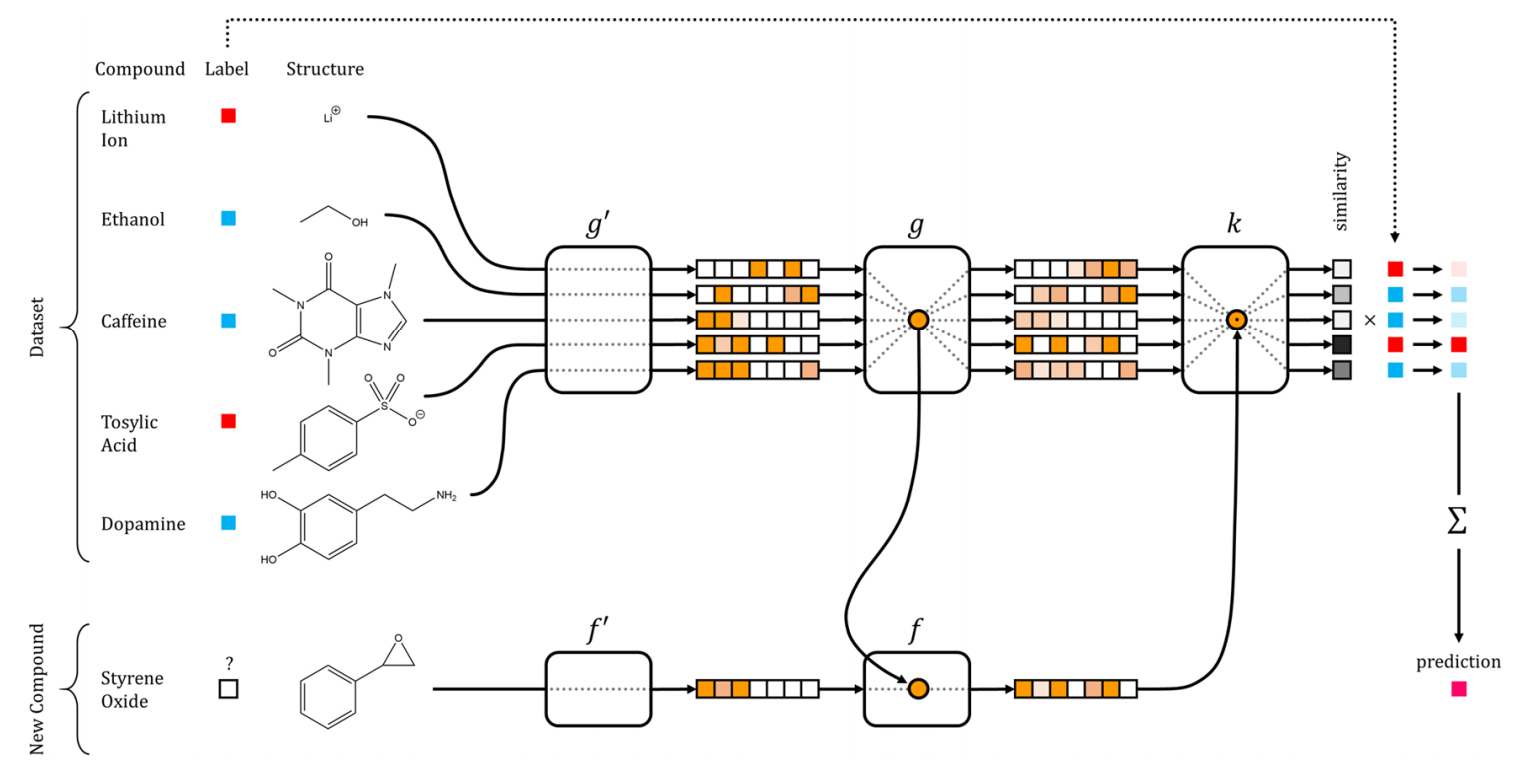
\includegraphics[width=0.9\linewidth]{img/pandeschematic.png}
	\caption[Schematic of one-shot learning in drug discovery]{Schematic of one-shot learning in drug discovery based on the Matching Network \citep{vinyals2016matching} architecture. Reproduced from \citet{altae2017low}.}
	\label{fig:schematiconeshotdrug}
\end{figure}

Their work is evaluation on the Tox21, the Side Effect Resource (SIDER) \citep{kuhn2016sider}, and MUV datasets\citep{rohrer2009maximum}. For every dataset, a subset of the targets is reserved for training and the rest for testing. Training is carried out as explained in the Matching Networks paper, in which training conditions match those at test time \citep{vinyals2016matching}. The authors make use of a Random Forest (RF) with 100 decision trees as a machine learning baseline model. They also utilise a conventional Graph Convolutional Networks (GCN)\citep{kipf2016semi} as an additional baseline model, which is trained using only a small support set from the test targets. They then experiment with Siamese Networks \citep{koch2015siamese}, Matching Networks \citep{vinyals2016matching}, and an adaptation of the Matching Networks by applying the iterative refinement concepts explained earlier.

The authors utilise ROC-AUC scores to report the performance of the models. Considering the extreme imbalance of the data in the utilised datasets, we note that the PR-AUC score would be a more appropriate evaluation measure. PR-AUC is based on the relationship between precision and recall, providing a clearer picture into how the model performs when predicting the \textit{positive} (active) class in the data. Predicting the ``active'' class correctly is of significant importance in virtual screening.

On the Tox21 and SIDER datasets, their proposed machine learning architecture achieves good ROC-AUC performance. The mean score for 10-shot learning on the median held-out task on Tox21 achieves a score of $0.823 \pm 0.002$, while for one-shot learning the model achieves a mean score of $0.827 \pm 0.001$. The reasons why one-shot learning achieved better performance than 10-shot learning is uncertain, as we expect the model to perform better with larger support sets. However, this might be attributed to variance in the data between experiments. On MUV data, the baseline machine learning models out-performed few-shot learning. The authors report that this is due to MUV data being maximally informative, and therefore structural similarity cannot be utilised to generalise for activity prediction. The authors open-sourced their models in the DeepChem library\citep{ramsundar2019deep}. However, the implementations are now outdated and not executable with the more recent versions of the DeepChem library, which makes reproduction of results difficult. However, we study the open-sourced implementation along with the implementation details in the original literature to successfully reproduce this work.
